\chapter{动态测试与静态分析结合的评测算法的实现与部署}
\label{cha:achievement}

在这一章节,会着重介绍本文的工作研究内容。中心内容为程序
填空题评测的算法的设计。

本章将先给出算法的选型,然后提出算法的结合设计以及算法流程,
之后详细说明算法在Matrix系统中实现的部署工作。

\section{算法的选择}
根据第二章介绍的算法选型,本文采用动态测试结合静态分析的评测思路,
对第二章提出的算法进行选择和结合,产生独有的程序评测算法。

首先,动态测试的算法选型上,采取基本动态测试算法。
基本动态测试算法对于答案简短的程序填空题效果良好,
可直接使用Matrix原生评测系统功能实现。
对于程序语法编译
错误导致无法进行动态测试,或者部分错误导致结果误差的情况,可
以交给静态分析去处理。

在静态分析的算法选型上,采用编辑距离算法。
编辑距离算法相比于分析语义的结合编译原理的相似度比对算法,
实现成本低,对应用的环境要求不大,不需要出题者进行复杂的
出题设置,不需要构建大量的语法规则。考虑到实验时时间的紧迫性,
,简单的编辑距离算法更符合现实需求。另一方面,
对于语言等价答案问题的处理,可通过设置多种标准答案以及动态
测试部分评测来解决。

本文的研究重点在于如何将动态测试与静态分析相结合,使得算法评测的分数更加接
近于人工的评测结果。

\section{程序填空评测问题算法的实现}
程序填空的评测功能实现的工作可以总结为以下五个方面:
\begin{enumerate}
  \item 评测流程的设计
  \item 评测算法的初步设计
  \item 系统交互方式的设计
  \item 以及题目数据的设计
  \item 各系统的部署
\end{enumerate}

\subsection{评测流程的设计}
程序填空题的评测流程广义上包括从出题到做题评分获取分数的整个完整的过程,大体的流程分为:
\begin{enumerate}
  \item 出题
  \item 做题
  \item 评测
  \item 分数查询
\end{enumerate}

\subsubsection{出题}

在Matrix系统中,题目以题库的形式存储在数据库以及文件系统,以便题目的
多次复用。出题后,老师和教学助理可以选择将题库的题目发布为课程的作业或者是
某场考试的题目。由于程序填空题包括动态和静态评测,因此出题需要提供的材料包
括题干本身、挖空的程序代码(填上标准答案可以完美执行出标准结果)、标准填空
答案以及相关的动态测试设置和相关的库代码文件。出题后、评测系统对标准答案进
行一次动态测试,以验证标准答案的正确性。

\subsubsection{做题}

题目作业开始或者对应考试开始后,学生登录Matrix应用系统,进行题目的阅
读并作答。此时若发布的作业或题目设置为评测定时(一般在考试场景),则提交后
不会马上给出评分。

\subsubsection{评测}

评测时机开始时,评测系统会在数据库中查找出学生提交的答案,并经过程序填空自动评测算法的
运行评测,得出评测分数,写入数据库。

\subsubsection{分数查询}

用户(老师、教学助理和学生)可通过系统查询权限内的学生的提交评测成绩。

\subsubsection{评测算法的初步设计}

评测算法采用动态测试的程序运行评测和静态的编辑距离算法相结合。

动态测试的技术实现在Matrix评测系统上已比较成熟,目前支持c和c++语言的评
测。通过评测系统原有的黑盒函数运行得出评测分数。

静态分析采用传统的编辑距离算法。下面为动态测试与静态分析结合的评测算法伪代码:

\begin{algorithm}[h]
\KwIn{学生提交的填空答案数组$Answers$}
\KwOut{$FinalGrade$}
\ForAll{填空答案数组$Answers$中的答案} {
  填入挖空的代码$Code$
}

对$code$进行动态测试,得出动态测试部分评分$DynamicGrade$

通过编辑距离算法相似度计算函数$EditDistanceSimilarity$
静态分析部分得分$StaticGrade = \sum_{i=0}^{n} EditDistanceSimilarity\left(Answer_i, StandardAnswer_i\right) * score_i$

最终得分 $FinalGrade = \max \left(DynamicGrade, StaticGrade\right)$

\caption{程序填空评测算法}
\label{algo:program_filling_algorithm}
\end{algorithm}

\subsection{系统交互方式的设计}
\label{sub:系统交互方式设计}
程序填空题评测依赖于 Matrix 应用系统,该系统包括 web 应用端、评测系统端
以及文件系统端、数据库及其它小型服务系统。web 应用、评测系统和文件系统和数
据库是核心,它们之间通过HTTP协议或数据库连接协议进行交互。主要系统的交互
联系如图\ref{fig:system_iteract}。

交互方式是根据算法与系统的应用结合,确定了交互方式,结合算法便可设计出
各系统交互的具体数据内容。

\begin{figure}[h]
  \centering
  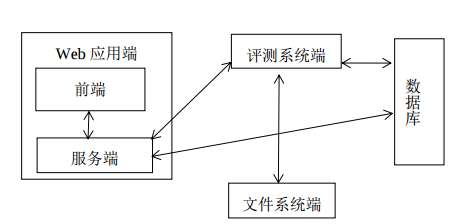
\includegraphics[width=0.5\textwidth]{image/chapter3/1}
  \caption{Matrix内部子系统交互}
  \label{fig:system_iteract}
\end{figure}


结合图\ref{fig:system_iteract}的交互和评测算法的流程,成功的交互流程可以分为以下几个步骤:

\begin{enumerate}
  \item 老师或TA通过前端发送出题信息到服务端
  \item 服务端将题目信息写入数据库,同时向评测系统发起评测请求,检验题目的正确性。
  \item 评测系统检验通过,向数据库写入题目数据。
  \item 老师或TA通过前端将题目发布到课程作业或者考试题目的请求发给服务端。
  服务端写入数据库,题目发布成功。
  \item 学生通过前端阅读题目,提交答案数据到服务端。
  \item 服务端将答案写入数据库,将填充了答案的完整代码发送到文件系统,并发送
  请求“通知”评测系统进行评测。
  \item 评测系统根据“通知”在数据库中找到对应提交答案代码的文件路径,再从文件系
  统中获取对应的答案代码进行评测,并将评测结果写入数据库。
  \item 用户(学生、老师、教学助理)通过前端获取题目的评测结果。
\end{enumerate}

\subsubsection{静态分析初期的交互设计产生的问题}
初期开发设计中,因与评测系统开发者的交互对接问题,静态分析部分的逻辑实现
写在了web服务端中。导致了动态测试和静态分析处理分离在了服务端和评测系统,
因此产生了异步问题。
根据算法\ref{algo:program_filling_algorithm},
题目最终的得分取动态测试和静态分析两者的分数中较大的分值,
因此最终得分需要等待动态测试和静态分析部分评测的完成。
由于这两部分的评测在服务端和评测系统分离运行,
难以确定两者完成的时间并计算出最终得分。
因此初期的策略为两部分的评测各自把分数写入
数据库,当前端向服务端查询分数时,服务端从数据库中查看两部分的分数,进行
计算得出最后得分并返回。

动态测试与静态分析的算法执行分离产生了两个问题,一是进行统计分数时无法直接读取
数据库,必须进行二次计算。二是将评测部分的逻辑代码写入负责业务逻辑的服务端
中不合规范。
因此后期通过与评测系统开发人员协调,将静态分析部分的评测实现迁移到了评
测系统,解决了异步处理问题,评测系统可以
控制两者完成的时间并计算出最终分数写入数据库。

\subsection{题目数据的设计}
程序填空题基于Matrix系统原有的编程题数据结构(用于动态测试),
增加以及程序填空特有的数据字段,当评测系统进行评测,会从
数据库查询获取对应题目的数据,从中获取评测需要的数据字段,
程序填空需要的数据字段包括动态测试部分和静态分析部分。

\subsubsection{动态测试部分的数据设计}
动态测试部分需要的数据字段为原有编程题数据结构中的字段,包括:
\begin{enumerate}
  \item grading: 编程检查每个阶段的分数,包括编译阶段、静态检查、标准测
试、随机测试、内存检查、Gtest 单元测试等。由于程序填空题不同于编程题,
用户不需要输入完整的代码,执行代码的变化十分有限,不必要设置多方面层次的评测,
因此默认只设置标准测试和随机测试的分数。
  \item language: 编程语言,现阶段支持 c 与 c++。
  \item standard\_language: 标准程序的编程语言。
  \item compliers: 对应不同语言的编译命令,该字段内容一般为固定,不需要用
户设置。
  \item limits: 程序运行限制的内存大小,该字段一般由出题者进行设置。由于填
空题的变化有限,一般取设定好的默认值。
  \item random:随机检查程序的编译命令和随机检查次数,编译命令一般固定,随
机检查次数由出题者进行设置。
  \item standard: 程序题对应的依赖代码文件的名称,包括 support(依赖的库文
件,显示在题目中)、hidden\_support(依赖的库文件,不显示)、random\_source
(随机数生成器代码文件,用于随机测试)、standard\_input(标准输入文件)、
standard\_output(标准输出文件)。
  \item submission: 学生提交的代码文件名。
  \item ouput\_program: 编译提交程序生成可执行文件的名字。
  \item entry\_point: 标准程序入口。
  \item standard\_score: 题目评测部分的满分。
  \item exec\_flag: 测试程序执行命令时附加的参数。
\end{enumerate}

以上是基本的程序评测需要的数据字段,但只有部分 grading、language、
standard\_lanugage、random、standard、submission、standard\_score 需要进行
设置。其余一般去设定的默认值。

\subsubsection{静态分析部分的数据设计}
静态分析部分,也是程序填空题基于编程题增加的数据字段,包括以下字段:

\begin{enumerate}
  \item standard\_answers: 填空的标准答案数组
  \item answer\_scores: 填空的分值设置数组,说明每一个空占的分值。
  \item code: 挖空关键填空的代码,其中需要填空的部分以字符串\$blank 表示
\end{enumerate}

\subsubsection{程序提交记录的数据设计}
学生提交答案时,服务端会将答案以提交记录的形式保存在数据库中,
评测系统评测时会根据评测请求给出的提交记录id,获取对应提交记录,
再根据提交记录关联的题目获取题目信息进行评测,提交记录中学生的答案
保存在detail字段中,
在detail 字段中,包含该字段:

student\_answers: 学生提交的填空答案,为字符串数组。

\subsection{各系统的部署}

\subsubsection{web前端的部署}
前端是web应用与用户交互的窗口,保持一个简洁明了舒适的前端界面,是一个
重要的工作。前端的工作就是将题目数据可视化显示给用户,
并收集用户交互的信息交给服务端处理。

程序填空题的用户交互中,前端部分核心为两个交互页面:出题页面和题目页面。

出题页面是老师出题的交互界面,分为题目、描述、挖空代码、填空标准答案、编程语言、题目相关文件、
时间内存要求、动态测试评测各阶段评分权重、标准输入输出样例和随机测试文件这
几个板块。板块页面图见附录图A-1到A-7。

题目页面,包含问题描述、答案提交和成绩反块板块,界面见附录图A-8至A-10。

前端包括HTML、CSS、Javascript文件的编写,前端除去页面样式(HTML、CSS)外,
需要在脚本代码(Javascript)完成获取用户填入的表单信息,当用户点击提交按钮,
将用户输入的表单信息通过http协议发送到服务端中处理的任务。

\subsubsection{web服务端的部署}
服务端需要完成以下几个任务:
\begin{enumerate}
  \item 接收前端发送的出题请求,将题目信息写入数据库,创建新题目。
  \item 接收前端发送的题目答案提交请求,将提交答案写入数据库,将填空答案填
入挖空代码形成完整的程序发送到文件系统储存,并向评测系统发送评测请求。
  \item 接收前端发送的成绩查询请求,从数据库中查询出成绩并返回到前端。
以上每个任务以对应的URL接口完成。
\end{enumerate}

服务端使用Node.js环境编写,使用express框架搭建服务器,
主要工作是以接口模块的形式完成上面的接口对应的逻
辑处理。

Matrix评测系统采用前后端分离的形式,对于页面、图片等静态资源的请求,
使用nginx服务器进行转发处理,服务端处理数据方面的api。对于程序填空题,
增加了查看题目信息、提交答案、查询题目分数的api。这些api对应的URL为:

\begin{enumerate}
  \item 查看题目信息(学生)/api/courses/:course\_id/assignments/\ GET
  \item 提交答案(学生)/api/courses/:course\_id/assignments/submission\ POST
  \item 查询最后一次提交记录(学生)/api/courses/:course\_id/assignments/submission/
  last\ GET
  \item 查看题库题目信息(老师、TA)/api/libraries/:library\_id/problem/:problem\_id\ GET
  \item 更新题库题目信息(老师、TA)/api/libraries/:library\_id/problem/:problem\_id\ POST
\end{enumerate}



具体处理逻辑的伪代码见算法\ref{algo:deal_submission}:

\begin{algorithm}[H]
\KwIn{浏览器端的答案提交请求报文}
\KwOut{返回的处理响应报文}
  检查报文提交格式
  \If{报文格式正确} {
    提取报文中学生填空答案。

    获取题目信息。

    将学生答案填入题目挖空代码,得到完整代码

    生成新的提交记录,写入数据库。

    将生成的代码发送至文件系统保存,与提交记录的id关联。

    向评测系统发送评测请求。

    向浏览器端发送成功提交的响应报文
  } \Else {
    向浏览器端发送错误信息的响应报文
  }
\caption{服务端对程序填空题提交请求的处理}
\label{algo:deal_submission}
\end{algorithm}

\subsubsection{评测系统的部署}
评测系统是部署程序填空评测系统的核心,主要的算法逻辑都在评测系统中执行,步骤如下:
\begin{enumerate}
  \item 首先评测系统接收到服务端发送的评测请求,根据发送的报文中的提交id,
  查询数据库找到对应的提交,获取提交的答案。
  \item 执行静态分析,将提交的答案与标准答案使用前面所述的静态分析算法计算
  出静态分析部分的评测得分。
  \item 根据提交的id从文件系统获取对应的动态测试的代码文件,进行动态测试,
  得出动态测试部分评测得分。
  \item 当两部分都评测完毕,取出两部分分数的较大分作为最终得分写入数据库。
\end{enumerate}

\section{程序填空评测的应用试验}

3.3.1 试验结果分析和存在问题
程序填空题的评测算法部署到Matrix应用系统后,在一场程序设计课程的期末
考试中进行了应用试验,图\ref{fig:prob_desc}为该考试某填空题的题目描述。
表\ref{fig:[prob_desc]}为部分的评
测结果。

题目包含四个填空,其标准答案依次为 int*,\ int、int\ *,const\ int*,\ int,\ int、
int*,\ int*、int*,\ int*。题目每空2分,总分8分。

\begin{figure}[h]
  \centering
  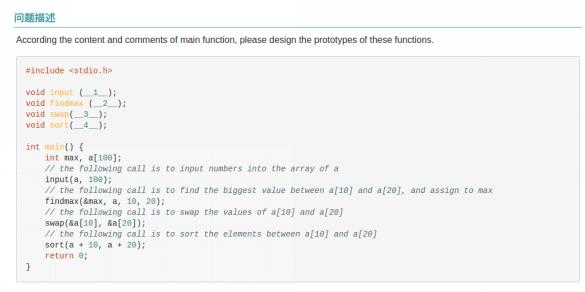
\includegraphics[width=0.5\textwidth]{image/chapter3/2}
  \caption{考试题目描述}
  \label{fig:prob_desc}
\end{figure}

\begin{table}[h] %voc table result
	\centering
	\caption{考试试验部分成绩统计}
	\begin{tabular}{*{4}{p{3cm}} *{3}{p{1cm}}}
		\toprule
		填空1答案 & 填空2答案 & 填空3答案 & 填空4答案 & 最终得分 & 动态测试得分 & 静态分析得分 \\
		\midrule
    Max & Max & Max & max & 0 & 0 & 0 \\
    int\ *,const\ int*,\ int,\ int & int\ *swap\_num, int\ *swap\_num1 & int*,\ int* & int\ *arr\_start,\ int *arr\_end & 3 & 0 & 3 \\
    int\ [],\ int & int\ *,\ int\ [],\ int,\ int & int\ *,\ int\ * & int*,\ int* & 7 & 0 & 7 \\
    int*,\ int & int\ *\ max,\ const\ int\ *\ const\ arr,\ const\ int\ start,\ const\ int\ end & int\ *\ a,\ int\ *\ b & int\ *\ const\ start,\ int\ *\ const\ end & 8 & 8 & 4 \\
		\bottomrule
	\end{tabular}
\end{table}


从评测结果统计看,可以看出问题如下:
\begin{enumerate}
  \item 动态评测对于大多数提交都是0分,
  没有起到评测作用。
\end{enumerate}

从考生答案的程序评测报告分析,发现问题在于第二个填空,对应
标准答案为 int*,const int*,\ int,\ int。
提交给评测系统的挖空代码(也是标准答案的测试代码),因防泄露答案(隐藏代码中含有答案),
实际上含有隐藏未公开给学生的部分,
实际的挖空代码中未显示给学生的部分如\ref{lst:hided_code}所示。

\begin{lstlisting}[caption=执行代码中未显示的部分,label=lst:hided_code,language=C]
void input(int* p, int n) {
    printf("input is OK\n");
}
void findmax(int * a, const int*b, int n, int m) {
    printf("findmax is OK\n");
}
void swap(int* x, int*y) {
    printf("swap is OK\n");
}
void sort(int *, int *) {
    printf("sort is OK\n");
}
\end{lstlisting}

可以看出,隐藏的代码片段\ref{lst:hided_code}是上面填空函数声明对应的定义实现,
若两者的参数类型不严格相
等,则会产生编译错误,而大多数考生的第二个填空的第二个参数漏了const声明,
导致整个代码无法通过编译。
因为一个填空的出错,导致所有的填空无法参与动态测
试,这是初期程序填空评测算法的一个重大缺陷。

另一方面,从题目上看,对于数组作为参数,
$int[]$这样的参数类型是可行的,但是由给出
的测试挖空代码来看,必须严格为指针类型才能视为正确答案。
这是出题过程的一个疏漏。

\section{本章总结}
本章说明了本文的主要工作。首先是程序填空算法的选型和设计,该部分的中心思想是
动态测试和静态分析算法的结合,如何将两部分的评测结果综合成一个最终得分。

然后是在Matrix评测系统中的实现部署,该部分内容的中心思想是算法与系统的结合,
根据算法流程设计数据结构和交互的报文数据内容。

同时也指出了算法在试验中存在的缺陷问题,问题包括题目的设计和算法的设计两个方面。
在下一章,将会说明评测算法的改进方案。

\clearpage
